% ------------------------------------------------------------------------------
% TYPO3 CMS 7.0 - What's New - Chapter "Deprecated Functions" (Russian Version)
%
% @author	Michael Schams <schams.net>
% @license	Creative Commons BY-NC-SA 3.0
% @link		http://typo3.org/download/release-notes/whats-new/
% @language	Russian
% ------------------------------------------------------------------------------
% LTXE-CHAPTER-UID:		4c309a81-71323cde-776eb944-4a8e5799
% LTXE-CHAPTER-NAME:	Deprecated Functions
% ------------------------------------------------------------------------------

\section{Устаревшие/удаленные функции}
\begin{frame}[fragile]
	\frametitle{Устаревшие/удаленные функции}

	\begin{center}\huge{Глава 5:}\end{center}
	\begin{center}\huge{\color{typo3darkgrey}\textbf{Устаревшие/удаленные функции}}\end{center}

\end{frame}

% ------------------------------------------------------------------------------
% LTXE-SLIDE-START
% LTXE-SLIDE-UID:		0f6f5195-bc41db71-f37a778e-791fe78b
% LTXE-SLIDE-ORIGIN:	c47248f9-03aa1da2-8dd9985d-762cf405 English
% LTXE-SLIDE-TITLE:		Legacy Layer
% LTXE-SLIDE-REFERENCE:	http://typo3.org/news/article/retaining-compatibility-to-typo3-cms6/
% ------------------------------------------------------------------------------

\begin{frame}[fragile]
	\frametitle{Устаревшие/удаленные функции}
	\framesubtitle{Слой совместимости}

	\begin{itemize}

		\item TYPO3 CMS 6.2: слой совместимости гарантирует работу старых расширений в новой базе кодов\newline
			\small
				Недостаток: снижение производительности (неполный потенциал системы)
			\normalsize

		\item TYPO3 CMS 7.0: слой совместимости удален из ядра\newline
			\small
				Следствие: старые расширения возможно не будут работать (например, расширения без области именования / namespaces)
			\normalsize

		\item Совместимость можно восстановить, установив системное расширение\texttt{EXT:compatibility6}
		\item Расширение будет в будущем перемещено в TER

	\end{itemize}

\end{frame}

% ------------------------------------------------------------------------------
% LTXE-SLIDE-START
% LTXE-SLIDE-UID:		718a9b96-22757c0e-da3328b4-83b77c4b
% LTXE-SLIDE-ORIGIN:	70da8aab-cd42e15f-fe254b81-41ceabb5 English
% LTXE-SLIDE-TITLE:		Backend User Management
% ------------------------------------------------------------------------------

\begin{frame}[fragile]
	\frametitle{Устаревшие/удаленные функции}
	\framesubtitle{Управление внутренними пользователями}

	\begin{itemize}
		\item Было удалено переключение на внутреннего пользователя ("режим поменять на")
	\end{itemize}

	\smaller\tabto{1cm}\begingroup\color{typo3red}TYPO3 CMS 6.2\endgroup\normalsize
	\begin{figure}\vspace{-0.4cm}
		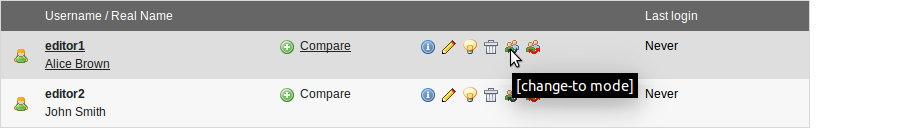
\includegraphics[width=0.90\linewidth]{DeprecatedRemovedFunctions/BackendUserSwitch1.png}
	\end{figure}

	\smaller\tabto{1cm}\begingroup\color{typo3red}TYPO3 CMS 7.0\endgroup\normalsize
	\begin{figure}\vspace{-0.4cm}
		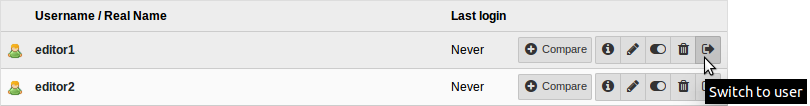
\includegraphics[width=0.90\linewidth]{DeprecatedRemovedFunctions/BackendUserSwitch2.png}
	\end{figure}

\end{frame}

% ------------------------------------------------------------------------------
% LTXE-SLIDE-START
% LTXE-SLIDE-UID:		dab03b2f-58fec033-16f931a9-f219aca5
% LTXE-SLIDE-ORIGIN:	10805d4d-787ce2f8-10e4329a-1451521a English
% LTXE-SLIDE-TITLE:		Removed Deprecated JavaScript Functions
% LTXE-SLIDE-REFERENCE:	https://github.com/TYPO3/TYPO3.CMS/commit/2dff81b963e1b77c7f068f91ffde73914a18b0be
% LTXE-SLIDE-REFERENCE:	https://forge.typo3.org/issues/62291
% LTXE-SLIDE-REFERENCE:	https://forge.typo3.org/projects/typo3cms-core/repository/revisions/9ac03e383e4786e868f4b1d81893e84c4621abc8/entry/typo3/sysext/core/Documentation/Changelog/master/Breaking-62291-RTEDeprecatedJavaScriptMethodsRemoved.rst
% ------------------------------------------------------------------------------

\begin{frame}[fragile]
	\frametitle{Устаревшие/удаленные функции}
	\framesubtitle{Удалены устаревшие функции JavaScript}

	\begin{itemize}
		\item В соответствие со \href{http://forge.typo3.org/projects/typo3v4-core/wiki/CoreDevPolicy}{стратегией устаревания},
			методы JavaScript, объявленных \textit{устаревшими} в TYPO3 CMS 4.7 были удалены, например:

		\begin{lstlisting}
			\TYPO3\CMS\Backend\Form\FormEngine->getSingleField_typeInput
			\TYPO3\CMS\Backend\Form\FormEngine->getSingleField_typeText
			\TYPO3\CMS\Core\Utility\GeneralUtility->quoted_printable
			\TYPO3\CMS\Core\Utility\GeneralUtility->encodeHeader
		\end{lstlisting}

		\smaller
			\texttt{HTMLArea.Editor.forceRedraw}\newline
				(используйте вместо этого \texttt{HTMLArea.Framework.doLayout})
				\vspace{0.2cm}

			\texttt{HTMLArea.Editor.convertNode}\newline
				(используйте вместо этого \texttt{HTMLArea.DOM.convertNode})
				\vspace{0.2cm}

			\texttt{HTMLArea.Editor.getBlockAncestors}\newline
				(используйте вместо этого \texttt{HTMLArea.DOM.getBlockAncestors})
		\normalsize

	\end{itemize}

\end{frame}

% ------------------------------------------------------------------------------
% LTXE-SLIDE-START
% LTXE-SLIDE-UID:		b488ced3-4db7472c-4baf87fb-907bb6d7
% LTXE-SLIDE-ORIGIN:	9da41efc-970e66a8-f9163c40-67cfa712 English
% LTXE-SLIDE-TITLE:		Removed Functions (1)
% LTXE-SLIDE-REFERENCE:	https://forge.typo3.org/issues/17579
% LTXE-SLIDE-REFERENCE:	https://forge.typo3.org/issues/62888
% ------------------------------------------------------------------------------

\begin{frame}[fragile]
	\frametitle{Устаревшие/удаленные функции}
	\framesubtitle{Удаленные функции (1)}

	\begin{itemize}

		\item
			\small
				Были удалены настройки TypoScript \texttt{config.uniqueLinkVar}\newline
				(теперь это поведение по умолчанию)
			\normalsize

		\item
			\small
				Удален проектор / ViewHelper
					\texttt{\textbackslash
						TYPO3\textbackslash
						CMS\textbackslash
						Documentation\textbackslash
						ViewHelpers\textbackslash
						Link\textbackslash
						Action}
				 (используйте вместо этого \texttt{f:be.buttons.icon} or \texttt{f:uri.*})
			\normalsize

		\item
			\small
				Удален параметр PageTSconfig \texttt{mod.web\_list.alternateBgColors}\newline
			\normalsize

		\item
			\small
				Удален PropertyMapper\newline
				(включая параметр \texttt{rewrittenPropertyMapper = 0})
			\normalsize

		\item
			\small
				Удалены условия TypoScript:

					\begin{itemize}
						\item\texttt{browser}
						\item\texttt{version}
						\item\texttt{system}
						\item\texttt{useragent}
					\end{itemize}
			\normalsize

	\end{itemize}

\end{frame}

% ------------------------------------------------------------------------------
% LTXE-SLIDE-START
% LTXE-SLIDE-UID:		a4192a18-eb25f914-9a72b29e-a539a839
% LTXE-SLIDE-ORIGIN:	efe86631-b6020ae8-ffa01160-6de29dc3 English
% LTXE-SLIDE-TITLE:		Removed Functions (1)
% ------------------------------------------------------------------------------

\begin{frame}[fragile]
	\frametitle{Устаревшие/удаленные функции}
	\framesubtitle{Удаленные методы (1)}

	Удалены следующие \textbf{методы}:

	\begin{itemize}
		\item
			\small
				\texttt{connectDB}\newline
				класса
				\texttt{\textbackslash
					TYPO3\textbackslash
					CMS\textbackslash
					Frontend\textbackslash
					Utility\textbackslash
					EidUtility}
			\normalsize
		\item
			\small
				\texttt{isDisplayCondition}\newline
				класса
				\texttt{\textbackslash
					TYPO3\textbackslash
					CMS\textbackslash
					Form\textbackslash
					FormEngine}
			\normalsize
		\item
			\small
				\texttt{int\_from\_ver}\newline
				класса
				\texttt{\textbackslash
					TYPO3\textbackslash
					CMS\textbackslash
					Core\textbackslash
					Utility\textbackslash
					GeneralUtility}
			\normalsize
		\item
			\small
				\texttt{getUniqueFields}\newline
				класса
				\texttt{\textbackslash
					TYPO3\textbackslash
					CMS\textbackslash
					Core\textbackslash
					DataHandling\textbackslash
					DataHandler}
			\normalsize

	\end{itemize}

\end{frame}

% ------------------------------------------------------------------------------
% LTXE-SLIDE-START
% LTXE-SLIDE-UID:		9606ed81-769ff8c8-50580212-91743470
% LTXE-SLIDE-ORIGIN:	293414d4-e87db3d5-afced471-ca9826ed English
% LTXE-SLIDE-TITLE:		Removed Methods (2)
% ------------------------------------------------------------------------------

\begin{frame}[fragile]
	\frametitle{Устаревшие/удаленные функции}
	\framesubtitle{Удаленные методы (2)}

	Удалены следующие \textbf{методы}

	\begin{itemize}

		\item
			\small
				\texttt{isSafeModeEnabled}\newline
				класса
				\texttt{\textbackslash
					TYPO3\textbackslash
					CMS\textbackslash
					Core\textbackslash
					Utility\textbackslash
					PhpOptionsUtility}
			\normalsize
		\item
			\small
				\texttt{registerSwiftMailer}\newline
				класса
				\texttt{\textbackslash
					TYPO3\textbackslash
					CMS\textbackslash
					Core\textbackslash
					Bootstrap}
			\normalsize
		\item
			\small
				\texttt{loadTCA}\newline
				класса
				\texttt{\textbackslash
					TYPO3\textbackslash
					CMS\textbackslash
					Core\textbackslash
					Utility\textbackslash
					GeneralUtility}
			\normalsize
		\item
			\small
				\texttt{isLocalconfWritable}\newline
				класса
				\texttt{\textbackslash
					TYPO3\textbackslash
					CMS\textbackslash
					Core\textbackslash
					Utility\textbackslash
					ExtensionManagementUtility}
			\normalsize

	\end{itemize}

\end{frame}

% ------------------------------------------------------------------------------
% LTXE-SLIDE-START
% LTXE-SLIDE-UID:		a7a85a5e-fa924610-9d1a43c5-4f6a66cd
% LTXE-SLIDE-ORIGIN:	a1ba1998-f88c1063-71470741-30b9f314 English
% LTXE-SLIDE-TITLE:		Removed Classes
% ------------------------------------------------------------------------------

\begin{frame}[fragile]
	\frametitle{Устаревшие/удаленные функции}
	\framesubtitle{Удаленные классы}

	Удалены следующие \textbf{классы}:

	\begin{itemize}

		\item
			\smaller
				\texttt{\textbackslash
					TYPO3\textbackslash
					CMS\textbackslash
					Backend\textbackslash
					Template\textbackslash
					MediumDocumentTemplate}
			\normalsize
		\item
			\smaller
				\texttt{\textbackslash
					TYPO3\textbackslash
					CMS\textbackslash
					Extbase\textbackslash
					Service\textbackslash
					TypeHandlingService}
			\normalsize

	\end{itemize}

\end{frame}

% ------------------------------------------------------------------------------
